\lab{Python}{NumPy Arrays and NumPy and SciPy}{NumPy Arrays and NumPy and SciPy} 
\objective{Create and manipulate powerful NumPy $n$-dimensional arrays and learn features available in NumPy and SciPy.}
\label{lab:NumPyArrays}

\section*{Why Use Arrays?} Python has a reasonably efficient list object, 
so why should we use arrays? Let's begin with a simple demonstration of why
arrays are important for numerical computation, in which
we will square a matrix that is represented as a two dimensional list (i.e. a list of lists). The lists form the rows of the matrix, and are "stacked" to form the columns; we obtain the elements of the jth column by taking the jth element of each row.

The following is a function that will accept two matrices, $A$ and $B$, and return $AB$ following the usual rules
of matrix multiplication. 

\lstinputlisting[style=fromfile]{arr_mult.py}

We can initialize a $k \times k$ array of integers like this:
\begin{lstlisting}
>>> k = 10 
>>> A = [range(i, i+k) for i in range(0, k**2, k)]
\end{lstlisting}

\section*{NumPy} NumPy is one of the fundamental packages for scientific
computing with Python. At its heart lies an efficient \li{ndarray}
object for fast computations. These $n$-dimensional arrays form
the foundation for all computations done in NumPy and SciPy (a
higher-level scientific computing library built on top of NumPy), and are a generalization of matrices. Just as a matrix (of dimension 2) can be thought of as a list of rows (of dimension 1), when we create an $n$-dimensional array, we create a list of arrays of dimension $n-1$. NumPy
is typically imported like this: 


\begin{lstlisting}
>>> import numpy as np
\end{lstlisting}


\begin{problem} 
Time how long the \li{arr_mult} function 
listed above and the NumPy method for matrix multiplication take to square matrices of size \li{k = 100, 200,}
and \li{300} and report the computed times. Briefly comment on the time needed to 
square a two dimensional list vs. a two dimensional NumPy array. 

Import timeit and NumPy. Create an array of the appropriate dimensions and square it, 
using both the function and the NumPy Method. (Be sure know the difference
 between doing element-wise multiplication and matrix multiplication).

In IPython you can time how long it takes for a line of code to execute
by prefacing it with \li{\%timeit}. If you aren't using IPython, you will need
to use the timeit function documented here: \url{https://docs.python.org/2/library/timeit.html}.

\end{problem}

% Below is a comparison of runtimes needed to square a matrix
% \begin{center} \begin{tabular}{|c|l|l|} \hline Data Structure & Size &
% Time (s) \\ \hline Python List & $1\times1$ & 0.0000181198 \\
% \cline{2-3} & $10\times10$ & 0.0002758503 \\ \cline{2-3} &
% $100\times100$ & 0.1336028576 \\ \cline{2-3} & $1000\times1000$ &
% 200.4009799957 \\ \hline \hline NumPy Array & $1\times1$ &
% 0.0000298023 \\ \cline{2-3} & $10\times10$ & 0.0000109673 \\
% \cline{2-3} & $100\times100$ & 0.0009210110 \\ \cline{2-3} &
% $1000\times1000$ & 2.1682999134 \\ \hline \end{tabular}
% %
% \end{center}
% 
% 
% 
The reason for the drastic speed difference is that Python, as a high
level interpreted language, tends to be slower than lower level compiled
languages such as C. The algorithms in NumPy are heavily optimized and
are usually implemented in C or Fortran. Instead of operating purely in
Python they use Python to run code that is written and optimized in
other, faster, languages. NumPy interfaces with some of the best packages
available for doing computational linear algebra and can be used to
write relatively fast programs.


\section*{Creating Arrays} The most elementary way to create an array is
to define it explicitly using \li{np.array()} (this creates a one dimensional array). 
\begin{lstlisting}
>>> a = np.array([0, 3, 8, 6, 3.14]) 
>>> a
array([0, 3, 8, 6, 3.14]) 
\end{lstlisting} 

NumPy provides a variety of
ways to easily create different kinds of arrays. \li{np.arange()}
creates a ranged array much the same way that Python's \li{range}
statement creates a list. \li{np.arange([start], stop, [step])} requires a
stop value, and can also take start and step values (optional). It returns the range
of evenly spaced values starting with the start value (default 0) and up to,
but not including, the stop value. 
\begin{lstlisting}
>>> b = np.arange(10) 
>>> b
array([0, 1, 2, 3, 4, 5, 6, 7, 8, 9]) 
\end{lstlisting}
 
We can also create an array of evenly spaced numbers over a desired interval.
This is done using \li{np.linspace(start, stop, num=50)} whose first
and second arguments define the endpoints of this closed interval while 
the third argument defines the number of samples. Note that the number
of samples defaults to 50. 
\begin{lstlisting}
# Return an array of 4 values ranging evenly from 0 to 32.
>>> c = np.linspace(0, 32, 4) 
>>> c
array([  0.        ,  10.66666667,  21.33333333,  32.        ])
\end{lstlisting} 


We can also create arrays that
consist entirely of ones or zeros using \li{np.ones()} and
\li{np.zeros()} respectively. 
\begin{lstlisting}
>>> d = np.ones(5) 
>>> d
array([ 1.,  1.,  1.,  1.,  1.])
\end{lstlisting} 

We can even create arrays using random values chosen
from a variety of probability distributions. These functions are stored
in a submodule of NumPy called \li{np.random}. 
\begin{lstlisting}
>>> e = np.random.rand(5) # uniformly distributed values 
>>> e
array([ 0.21845499,  0.73352537,  0.28064456,  0.66878454,  0.44138609])
# Return an array of 6 randomly generated integers uniformly
# distributed in [0, 5).
>>> f = np.random.randint(0, 5, 6) 
>>> f
array([ 3,  1,  0,  3,  4,  1])

\end{lstlisting} 

We can also allocate an array without initializing its
values. This is most useful when the initial values of an
array do not matter (like when you are constructing an array filled with
specific values or when you are going to overwrite it).
\begin{lstlisting}
>>> g = np.empty(5) 
>>> g
array([  0.00000000e+000,   1.30586451e-316,   1.17126324e-316,
0.00000000e+000,   2.37151510e-322]) 
\end{lstlisting} 

We can also create an array with the same shape and type as another given array. 
To verify this we can check the shape and data type of both arrays. More information
on \li{shape} and \li{dtype} will be provided shortly.
\begin{lstlisting}
# Note that 2,3 dictates a 2 by 3 array of random values
>>> h = np.random.rand(2,3) 
>>> h.shape
(2,3)
>>> h.dtype
dtype('float64')
>>> j = np.empty_like(h)
>>> j.shape
(2,3)
>>> j.dtype
dtype('float64')
\end{lstlisting} 
Note that you can also dictate that your new array be
filled entirely with ones or zeros by using the \li{np.ones_like} or
\li{np.zeros_like}, respectively.


\section*{Array Objects} 
Unlike Python containers, all of the elements
of an array must have the same data type. These datatypes are
machine-native data types that avoid the overhead (time consumption and inefficiency)
 of Python objects. For example,  an \li{int} in NumPy is not the same as an \li{int} in Python;
the \li{int} data type native to NumPy stores integers in a way that uses less processor power to handle. The benefit
of using these machine-native types is a tremendous speedup of
numerical operations. Datatypes supported by NumPy are shown in Table \ref{numpytypes}.
\begin{table} 
\begin{tabular}{l|l} 
Data type & Description 
\\ \hline 
\li{bool} & Boolean \\ 
\li{int8} & 8-bit integer \\ 
\li{int16} & 16-bit integer \\ 
\li{int32} & 32-bit integer \\
\li{int64} & 64-bit integer \\ 
\li{int} & Platform integer (depends on platform) \\ 
\li{uint8} & Unsigned 8-bit integer \\ 
\li{uint16} & Unsigned 16-bit integer \\ 
\li{uint32} & Unsigned 32-bit integer \\
\li{uint64} & Unsigned 64-bit integer \\ 
\li{float16} & Half precision float \\ 
\li{float32} & Single precision float \\ 
\li{float64} & Double precision float (also \li{float}) \\ 
\li{complex64} & Complex number represented by two single precision floats \\ 
\li{complex128} & Complex number represented by two double precision floats (also \li{complex})
\end{tabular} 
\caption{Native numerical data types available in NumPy.}
\label{numpytypes} 
\end{table} 

Like any other object in Python, \li{ndarray} objects have methods and properties associated with them. 
We can derive information from arrays by looking at their different attributes. The data type of the array
 is stored in the \li{dtype} property. Many of the array constructors accept an optional
\li{dtype} keyword that lets you specify the data type of the array to be created. 

\begin{lstlisting}
>>> a.dtype
dtype('float64')
>>> a = np.array(range(5), dtype=np.uint8) 
>>> a.dtype
dtype('uint8') 
\end{lstlisting} 

We can check the number of dimensions an
array has by looking at the value of the \li{ndim} property. 
\begin{lstlisting}
>>> a.ndim
1 
\end{lstlisting} 

We can see the sizes of each dimension by looking at
the \li{shape} property. This will return a Python tuple of the size of
each dimension. 
\begin{lstlisting}
>>> a.shape
(5,)
# Return the size of the first dimension.
>>> a.shape[0]
5 
# Return the total number of elements in the array.
>>> a.size 
5
\end{lstlisting} 

For a single dimensional array, these properties are
uninteresting. However, these array properties are the most efficient way 
to understand the size and shape of an array.

Let's look at higher dimensional arrays. One, two, and three dimensional
arrays are easy to visualize. As previously mentioned, higher dimensional NumPy arrays can simply be
thought of as arrays within arrays. A three dimensional array can just
be thought of as an array of two dimensional arrays, or an array of arrays of (one dimensional) arrays. The 3D index, \li{A[3, 5,
1]}, essentially means \emph{take the second element} \li{(1)} \emph{of the sixth
subarray} \li{(5)} \emph{of the fourth subarray} \li{(3)} \emph{of A}. 
 Each dimension is called an \emph{axis} in NumPy (ie. a 3D array has 3 axes).  
In a 2D array, we may refer to the rows as the zero axis and the columns as the
one axis. Many of NumPy's functions can be restricted to an axis. 

Most of the array constructors we have considered thus far support 
creating arrays with an arbitrary number of dimensions. However, some are restricted to lower dimensions, making them convenient for matrix operations; for example, we can easily create an identity matrix with \li{np.eye}, \li{np.identity},
 or \li{np.diag}. 
 
\li{np.eye} is the most versatile of these methods and allows for non-square outputs, 
in which case it puts ones on the diagonal and zeros everywhere else. 
\li{np.diag} is an interesting function.  If given an existing 2D array, 
it will extract the diagonal elements and return a 1D array. However, if given 
a 1D array or a list, it will construct a 2D array with the list elements as the diagonal.

\begin{lstlisting}
>>> h = np.eye(3) 
>>> h
array([[ 1.,  0.,  0.],
       [ 0.,  1.,  0.],
       [ 0.,  0.,  1.]])
>>> np.eye(3, 4)
array([[ 1.,  0.,  0.,  0.],
       [ 0.,  1.,  0.,  0.],
       [ 0.,  0.,  1.,  0.]])
>>> np.identity(3)
array([[ 1.,  0.,  0.],
       [ 0.,  1.,  0.],
       [ 0.,  0.,  1.]])
>>> np.diag(h)
array([ 1.,  1.,  1.])
>>> i = np.diag(np.arange(5))
>>> i
array([[0, 0, 0, 0, 0],
       [0, 1, 0, 0, 0],
       [0, 0, 2, 0, 0],
       [0, 0, 0, 3, 0],
       [0, 0, 0, 0, 4]])
\end{lstlisting} 

Another powerful function is
\li{np.tile()}. Tiling allows us to construct an arbitrary-dimensional array by repeating an existing array
 in a specified pattern. \li{np.tile()} allows us to tile arrays across one or more dimensions. 
\begin{lstlisting}
>>> j = np.array([1, 9, 5, 2])
# Repeat j three times in the first dimension 
np.tile(j, 3)
array([1, 9, 5, 2, 1, 9, 5, 2, 1, 9, 5, 2])
# Make an array of three lists (third dimension) of three lists 
# (second dimension) of two copies of j each (first dimension)
>>> k = np.tile(j, (3, 3, 2)) 
>>> k
array([[[1, 9, 5, 2, 1, 9, 5, 2],
        [1, 9, 5, 2, 1, 9, 5, 2],
        [1, 9, 5, 2, 1, 9, 5, 2]],

       [[1, 9, 5, 2, 1, 9, 5, 2],
        [1, 9, 5, 2, 1, 9, 5, 2],
        [1, 9, 5, 2, 1, 9, 5, 2]],

       [[1, 9, 5, 2, 1, 9, 5, 2],
        [1, 9, 5, 2, 1, 9, 5, 2],
        [1, 9, 5, 2, 1, 9, 5, 2]]])

\end{lstlisting}


We often find it useful to create arrays that represent a
two-dimensional grid of coordinates. This is done using the
\li{meshgrid()} function, for example:
\begin{lstlisting}
>>> x = np.arange(4) 
>>> y = np.arange(4, 8) 
>>> X, Y = np.meshgrid(x, y) 
>>> X
array([[0, 1, 2, 3],
       [0, 1, 2, 3],
       [0, 1, 2, 3],
       [0, 1, 2, 3]])
>>> Y
array([[4, 4, 4, 4],
       [5, 5, 5, 5],
       [6, 6, 6, 6],
       [7, 7, 7, 7]])
\end{lstlisting} 
As you can see, \li{X} is an array representing the $x$-coordinates for a 4x4 grid of points and \li{Y} is an array representing the
$y$-coordinates of that same grid of points. For example, the (0,0) entries in X and Y correspond to the point (0,4), the (2,3) entries correspond to the point (3,6), and so on.

\begin{comment} 
When
creating large grids of points this can use large amounts of RAM, so the
meshgrid function includes the \li{copy} argument which, when set to
false, returns arrays that are views of the original arrays instead of
copies (views and copies are discussed later in this lab). For example,
instead of running \li{np.meshgrid(x, y)} you could run
\li{np.meshgrid(x, y, copy=False)}. This can be much faster, but should
probably only be used if you do not intend to make any additional
changes to the coordinates grid independent of the values stored in the
original arrays.

Every NumPy array has five flags that give important information about
the array. We can check if an array is read-only by looking at its
flags, or we can check how the array's contents are laid out in memory.
Only the \texttt{WRITEABLE} and \texttt{ALIGNED} flags can be modified. 
The other flags are read-only. The \texttt{OWNDATA} flag lets us know if
the array is a view or not. We will explain array views later in this
lab. \begin{lstlisting}
>>> i.flags
  C_CONTIGUOUS : True F_CONTIGUOUS : False OWNDATA : True WRITEABLE :
  True ALIGNED : True UPDATEIFCOPY : False \end{lstlisting} NumPy has
  two different memory orderings for an array. Many array constructors
  allow you to specify an \li{order} keyword that determines the memory
  layout of the array. \begin{description} \item[Row-major:] Arrays are
  stored by rows in continuous memory. Languages such as C and Python
  use row-major indexing. NumPy arrays by default use this indexing
  convention. When an array is stored in memory the addresses to its
  values are stored linearly. In simplest terms, the ordering of an
  array determines whether its rows or its columns are stored in
  contiguous blocks (for example: row 0, row 1, row 2, ... as opposed to
  column 1, column 2, column 3, ...). For an array where the rows are in
  contiguous blocks in memory, performing any sort of operation along a
  column will be slower than performing that same operation along a row
  of the same length. This difference is because of the irregular memory
  access pattern. In NumPy, row-major arrays are identified as \emph{C
  contiguous} (\li{order=`C'}). \item[Column-major:] Arrays are stored
  by columns in contiguous memory. Languages like FORTRAN, MATLAB, and R
  use column-major indexing. For a column major array, operations that
  run along rows are slower. In NumPy, column-major arrays are
  identified as \emph{FORTRAN contiguous} (\li{order=`F'}).
  \end{description} Paying attention to how your arrays are indexed will
  be beneficial to the performance of your algorithms. Speed is not
  usually a critical concern, but it is good to know these things when
  speed does become an issue.

% \section*{Iterating Through Arrays} Iterating through an array
% mitigates most, if not all, speed advantages of NumPy. The advantage
% of NumPy is that all of the iterating has been pushing into the highly
% efficient looping structures of C or Fortran. Implementing that loop
% in Python dramatically slows down the speed of execution. There are
% however some valid cases where iterating over the array is necessary.
% NumPy provides several efficient iterators that can be used in such
% instances.
% 
\end{comment}

\section*{Iterating Through Arrays} Iterating through an array
mitigates most, if not all, speed advantages of NumPy. The advantage
of NumPy is that all of the iterating has been pushing into the highly
efficient looping structures of C or Fortran. Implementing that loop
in Python dramatically slows down the speed of execution. There are
however some valid cases where iterating over the array is necessary.
NumPy provides several efficient iterators that can be used in such
instances.

\section*{Array Views and Copies} It is important to understand that
NumPy has two ways of returning an array. Slice operations always return
a \emph{view} and fancy indexing always returns a \emph{copy}.
Understand that even though they may look the same, views and copies are
very different.

Views are special arrays that are unique objects, but reference the same memory as the array they 
reference; changing elements in a view also changes the array it references. 
Below, we demonstrate the behavior of a view. Notice that \li{m} looks like a copy
of \li{k} even though it is not. 
The \li{np.reshape()} method will be discussed in greater detail 
further on in this lab.
\begin{lstlisting}
>>> k = np.reshape(np.arange(25), (5,5)) 
>>> k
array([[ 0,  1,  2,  3,  4],
       [ 5,  6,  7,  8,  9],
       [10, 11, 12, 13, 14],
       [15, 16, 17, 18, 19],
       [20, 21, 22, 23, 24]])
# Although m appears to be a copy of k, it is actually a view. 
>>> m = k[:]
>>> m
array([[ 0,  1,  2,  3,  4],
       [ 5,  6,  7,  8,  9],
       [10, 11, 12, 13, 14],
       [15, 16, 17, 18, 19],
       [20, 21, 22, 23, 24]]) 
# This indicates that m and k are unique objects.
>>> id(m) == id(k) 
False
# Change the third element of m (itself a list) to 500
>>> m[2] = 500 
>>> m
array([[  0,   1,   2,   3,   4],
       [  5,   6,   7,   8,   9],
       [500, 500, 500, 500, 500],
       [ 15,  16,  17,  18,  19],
       [ 20,  21,  22,  23,  24]])
# Changing m also changed k.
>>> k 
array([[  0,   1,   2,   3,   4],
       [  5,   6,   7,   8,   9],
       [500, 500, 500, 500, 500],
       [ 15,  16,  17,  18,  19],
       [ 20,  21,  22,  23,  24]])
\end{lstlisting} 

The reason that changing the array \li{m} also changed
the array \li{k} is because \li{m} and \li{k} contain references to the
same data in memory, even though they are different Python objects.
Views reduce the overhead of making copies of arrays and are useful when
we want to change certain parts of the array.

A copy of an array is a separate array with its own memory. An array can
be copied using the \li{np.copy()} function (also available as a method of 
the array object). 

\begin{lstlisting}
>>> j = np.reshape(np.arange(25), (5,5))
>>> n = np.copy(j) 
# We still have unique objects.
>>> id(n) == id(j) 
False
>>> n[2] = 500 
>>> n
array([[  0,   1,   2,   3,   4],
       [  5,   6,   7,   8,   9],
       [500, 500, 500, 500, 500],
       [ 15,  16,  17,  18,  19],
       [ 20,  21,  22,  23,  24]])
>>> j
array([[ 0,  1,  2,  3,  4],
       [ 5,  6,  7,  8,  9],
       [10, 11, 12, 13, 14],
       [15, 16, 17, 18, 19],
       [20, 21, 22, 23, 24]])
# Fills the values of an existing array, j, with n.
>>> j[:] = n
>>> j
array([[  0,   1,   2,   3,   4],
       [  5,   6,   7,   8,   9],
       [500, 500, 500, 500, 500],
       [ 15,  16,  17,  18,  19],
       [ 20,  21,  22,  23,  24]])
\end{lstlisting} 
Changing the data in a copy of an array does not affect the data in the 
original array because the two arrays have different locations in memory.

\section*{Indexing and Slicing} Every element of an array has a unique
numeric address, or index, that can be used for accessing that element. "Indexing" 
refers to the methods we use to access elements with specified indices.
All indices in Python and NumPy starts with \li{0} as the first value. 
Negative indexing can also be used for NumPy arrays. 
\begin{lstlisting}
>>> a = np.arange(3, 9) 
>>> a[0]
3
# Return the last element of a; a[-2] would return the second to last element
>>> a[-1]
8 
\end{lstlisting} 
When indexing a multidimensional array, it might be
tempting to use the \li{f[i][j][k]} form of indexing. This is a \emph{very}
inefficient way to access NumPy arrays. NumPy has provided an optimized
indexing syntax in which the precise index is expressed as a tuple (the
\li{k[i,j,k]} form).  This optimized indexing becomes significantly
faster when we work with arrays of more than one dimension. The reason that the
unoptimized \li{f[i][j][k]} indexing is slow is that each bracket is returning an
array slice. For a 3D array, \li{k[0][0][0]} will create temporary
slices of \li{k} from each dimension (\li{k[0]}, \li{k[0][0]}, and
\li{k[0][0][0]}) and return the last slice. Using tuples as indices allows
NumPy to access the element directly (without creating intermediate slices 
along the way), which is much more efficient.

It is also possible to index an array with an object such as a list or
an array instead of requesting slices with specified indices, but in this case 
NumPy behaves a little differently. This feature is commonly referred to as fancy
indexing. One difference is that fancy indexing always returns a copy of an array
instead of a view. 
There are two types of fancy indexing: boolean and integer. 
Boolean indexing uses an array of \li{True} or \li{False} values to 
determine which elements of the array to take. 
\begin{lstlisting}
>>> b = np.arange(25).reshape((5,5)) 
>>> b
array([[ 0,  1,  2,  3,  4],
       [ 5,  6,  7,  8,  9],
       [10, 11, 12, 13, 14],
       [15, 16, 17, 18, 19],
       [20, 21, 22, 23, 24]])
# We refer to this array as "bmask" because we are "masking" the
# values not specified instead of deleting them.
>>> bmask = (b > 15) & (b < 23) 
# Note that logic operations on arrays result in true-false valued arrays.
>>> bmask 
array([[False, False, False, False, False],
       [False, False, False, False, False],
       [False, False, False, False, False],
       [False,  True,  True,  True,  True],
       [ True,  True,  True, False, False]], dtype=bool)
>>> b[bmask]
array([16, 17, 18, 19, 20, 21, 22])
# This is the condensed form. 
>>> b[(b > 15) & (b < 23)] 
array([16, 17, 18, 19, 20, 21, 22])
>>> b[~bmask] # invert the mask
array([ 0, 1, 2, 3, 4, 5, 6, 7, 8, 9, 10, 11, 12, 13, 14, 15, 23, 24])
# Return an array of elements b[0,0], b[2,2], and b[4,4].
>>> b[(0, 2, 4), (0, 2, 4)] 
array([ 0, 12, 24])
# This is the same as above, but with ranges instead of tuples; 
# the range(0, 5, 2) is equivalent to the tuple (0, 2, 4).
>>> b[range(0, 5, 2), range(0, 5, 2)] 
array([ 0, 12, 24])
# Take the first (0) and last (-1) columns. Note that this is a list of discrete
# indices, not a slice. The : indicates a slice including all of that axis.
>>> b[:, [0, -1]]  
array([[ 0,  4], [ 5,  9], [10, 14], [15, 19], [20, 24]])
\end{lstlisting}

Though fancy indexing does not return a view of an array, it \emph{can}
be used for assignment. For example, we can set all values of an array
that are less than \li{.5} to \li{0} in the following way: 
\begin{lstlisting}
>>> from numpy.random import rand 
>>> A = rand(10, 10) 
>>> A[A<.5] = 0.
\end{lstlisting}

Slicing an array is very similar to slicing a Python list. An array
slice returns some subset of an array. We can access ranges of elements
using Python lists. We can also more concisely select ranges using the
\li{array[start:stop:step]} range notation. 
\begin{lstlisting}
>>> k = np.arange(25).reshape((5,5)) 
>>> k
array([[ 0,  1,  2,  3,  4],
       [ 5,  6,  7,  8,  9],
       [10, 11, 12, 13, 14],
       [15, 16, 17, 18, 19],
       [20, 21, 22, 23, 24]])
# Return every other element of the rows and every third element of
# the columns.  
>>> k[::2, ::3] 
array([[ 0,  3],
       [10, 13],
       [20, 23]])
# Reverse the order of the columns; the : indicates a slice including
# all of that axis.
>>>k[:, ::-1] 
array([[ 4,  3,  2,  1,  0],
       [ 9,  8,  7,  6,  5],
       [14, 13, 12, 11, 10],
       [19, 18, 17, 16, 15],
       [24, 23, 22, 21, 20]])
# Extract the lower right 2x2 subarray.
>>> k[3:, 3:] 
array([[18, 19],
       [23, 24]])
# Extract the second column. The returned array is 1D.
>>> k[:, 1] 
array([ 1,  6, 11, 16, 21]) 
\end{lstlisting} 

Operations like those above
are examples of array slicing. Array slices are views, not copies, of
portions of the data of the original array.

% \begin{problem} Generate a random $1000 \times 1000$ array \li{A}. Now
% create an uninitialized array \li{B} with all the same attributes as
% \li{A}. Now do the following 100 times: \begin{itemize} \item
% Overwrite \li{B} so that it is an array of new random values like
% \li{A}. This can be done like this: \li{B[:] = rand(1000,1000)} \item
% Use fancy indexing to make \li{A} the maximum of \li{A} and \li{B}.
% \end{itemize} Now take \li{exp(A)} and have NumPy store the output
% directly in \li{A}. Take the maximum along the vertical axis and
% average the result. The final number should be very close to $e$.
% \end{problem}
% 
\section*{Manipulating Arrays} NumPy provides a variety of functions for
working with already existing arrays. The shape of a NumPy array can be
changed by using the \li{np.reshape()} function (also available as a
method of array objects). The reshape function gives an array a new
shape without changing the data of the array. It is imperative that 
the new shape be compatible with the size of the array. 
It returns a view whenever possible, otherwise it will return 
a copy of the reshaped array.
\begin{lstlisting}
>>> k = np.arange(36)
array([ 0,  1,  2,  3,  4,  5,  6,  7,  8,  9, 10, 11, 12, 13, 14, 15, 16, 17, 18, 19, 20, 21, 22, 23, 24, 25, 26, 27, 28, 29, 30, 31, 32, 33, 34, 35])
>>> k.shape
(36,)
>>> k.reshape((12, 3))
array([[ 0,  1,  2],
       [ 3,  4,  5],
       [ 6,  7,  8],
       [ 9, 10, 11],
       [12, 13, 14],
       [15, 16, 17],
       [18, 19, 20],
       [21, 22, 23],
       [24, 25, 26],
       [27, 28, 29],
       [30, 31, 32],
       [33, 34, 35]])
\end{lstlisting} 
Sometimes it is best to work on the entire array in single dimension. 
We can reshape the array to a single dimension, or use \li{np.ravel}. 
The \li{flat} method is an iterator that will iterate over a 
flattened array efficiently.
\begin{lstlisting}
>>> k.ravel()
array([ 0,  1,  2,  3,  4,  5,  6,  7,  8,  9, 10, 11, 12, 13, 14, 15, 16, 17, 18, 19, 20, 21, 22, 23, 24, 25, 26, 27, 28, 29, 30, 31, 32, 33, 34, 35])
# The -1 in the axis tells NumPy to make the axis as long as is necessary.
>>> k.reshape((-1,)) 
array([ 0,  1,  2,  3,  4,  5,  6,  7,  8,  9, 10, 11, 12, 13, 14, 15, 16, 17, 18, 19, 20, 21, 22, 23, 24, 25, 26, 27, 28, 29, 30, 31, 32, 33, 34, 35])
>>> timeit k.ravel()
1000000 loops, best of 3: 291 ns per loop
>>> timeit k.reshape((-1,))
1000000 loops, best of 3: 418 ns per loop 
\end{lstlisting} 
The transpose \li{np.T} is another efficient NumPy operation that returns an array
view. 

\begin{lstlisting}
>>> b = np.arange(16).reshape((4,4)) 
>>> b.T
array([[ 0,  4,  8, 12],
       [ 1,  5,  9, 13],
       [ 2,  6, 10, 14],
       [ 3,  7, 11, 15]])
\end{lstlisting}

\begin{comment}

We can also manipulate the axes of an existing array using
\li{np.swapaxes} and \li{np.rollaxis}. Functions can also be applied
across one or more axes using \li{np.apply_across_axis} or
\li{np.apply_across_axes}. The function \li{np.unique} will return the
sorted unique elements of the input array. There are also methods for
constructing arrays from individual subarrays. While they may be useful,
use them very carefully as they can have a very negative impact on
performance. Functions like \li{np.hstack} and \li{np.vstack} will
horizontally or vertically stack the input arrays into a new NumPy
array.

\end{comment}

\begin{problem} 
Operations that create completely new arrays are often slower than 
operations that create views because allocating an array can be time 
consuming. 
\begin{enumerate}
\item Create an $1000 \times 1000$ array \li{A} of random floating point values. 
\item Compare the speed of the operations \li{A.reshape(A.size)}
and \li{A.flatten()}. Note that we are calling the methods of the arrays. 
They are the same as \li{np.reshape(A, A.size)}, and \li{np.flatten(A)}
respectively. 
\item Why is there such a difference in speed? 
\end{enumerate}
\end{problem}

\begin{problem} 
One good application of array slicing is the Jacobi
method for solving Laplace's equation, which is used to model
steady-state heat flow on a square. This is an example of a simple
iterative method. In this case we will modify our array in place. 
\begin{enumerate}
\item Make a function that accepts an array and a tolerance as input and does the
following: 
\item Make a copy of the array. 
\item Create a variable to track the difference between the arrays. Initialize
it as the tolerance parameter your function accepts. 
\item While the difference is greater than or equal
to the tolerance 
\begin{enumerate} 
\item set all points that are not on an edge of the new array equal to the average of their 4 immediate neighbors. Use the values from the old array for this computation. 
This should only take one line and should be based entirely on array slicing, NOT iterating through the array.
(Hint: given a 2D array \li{A}, the slice \li{A[1:-1,1:-1]} references
all non-edge entries, \li{A[:-2,1:-1]} references the upper neighbors,
and \li{A[1:-1,2:]} references the right neighbors.) 
\item update the difference to be the maximum of the absolute value of the new array
minus the old one. 
\item copy the values from the new array into the old
one (without creating a new array). 
\end{enumerate} 
\end{enumerate}

Now use the following code to generate a plot of your results
\lstinputlisting[style=fromfile]{laplace_plot.py} 
It should resemble the following figure.

\begin{figure} [H]
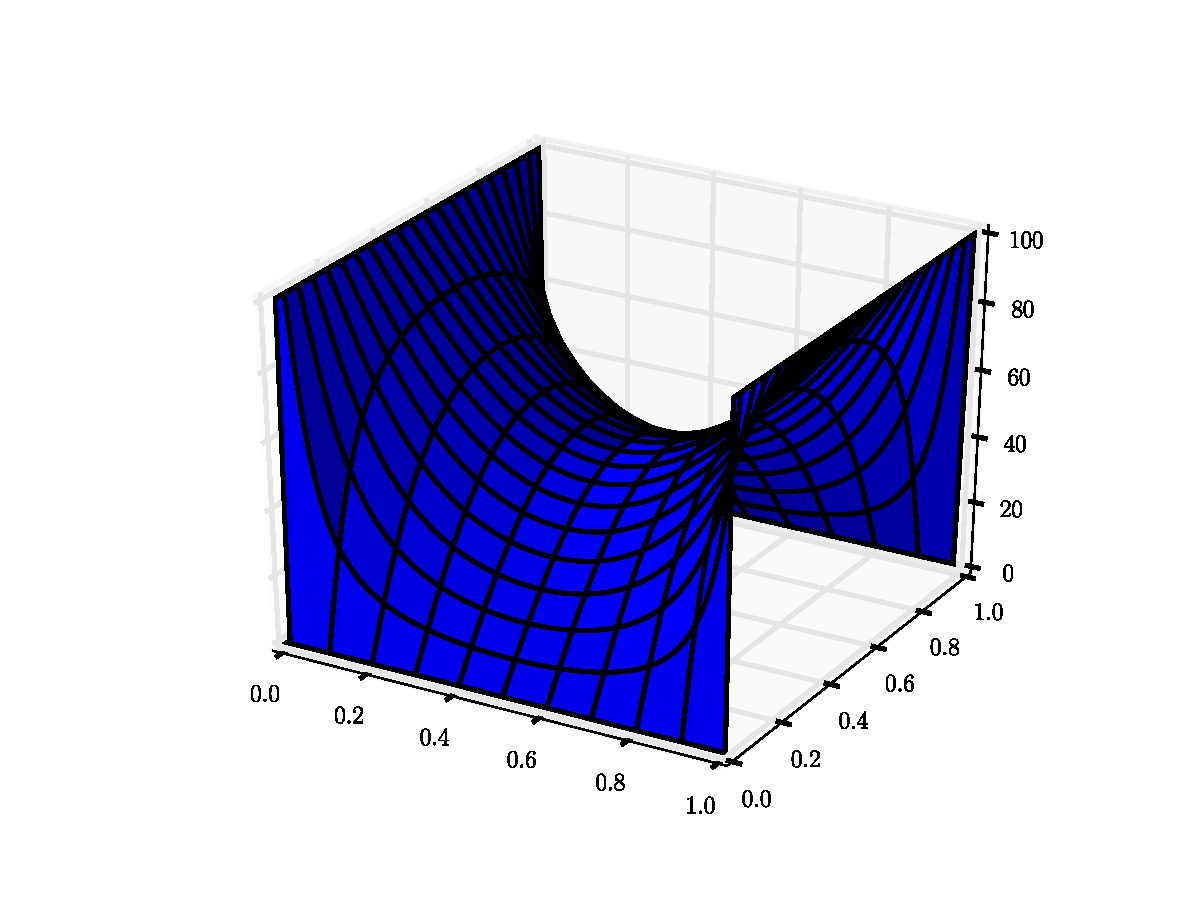
\includegraphics[width=.75\textwidth]{laplace.pdf}
\end{figure} 
\end{problem}

\section*{Logical Operations} 
Logical operations return arrays of only true or false values. 
These arrays are often useful in masking values in other arrays. 

\begin{lstlisting}
>>> a = np.random.rand(5,5) 
>>> a<.5
array([[False,  True,  True, False, False],
       [False,  True,  True, False,  True],
       [ True,  True,  True,  True,  True],
       [False,  True,  True, False, False],
       [ True,  True, False, False, False]], dtype=bool)
>>> a[a<.5]
array([ 0.30726555,  0.45395769,  0.05825412,  0.04896835,  0.02053107,
        0.33587884,  0.14637301,  0.2109408 ,  0.13908897,  0.12292625,
        0.24329939,  0.053114  ,  0.40227096,  0.21899495])
>>> a[a<.3] = 0 
>>> a
array([[ 0.90428049,  0.30726555,  0.45395769,  0.99935736,  0.96856189],
       [ 0.69711146,  0.        ,  0.        ,  0.88489964,  0.        ],
       [ 0.33587884,  0.        ,  0.        ,  0.        ,  0.        ],
       [ 0.75447365,  0.        ,  0.        ,  0.58333895,  0.67131309],
       [ 0.40227096,  0.        ,  0.60919998,  0.94026012,  0.52745694]])
\end{lstlisting} 
All the comparison operators can be used like this when working with arrays. 
We can quickly test if \emph{all} elements of a given axis
evaluate to true with \li{np.all}.  
Likewise, we can test if \emph{any} element evaluates to true with 
\li{np.any}. 

Most floating point numbers cannot be represented perfectly 
as a binary fraction and are thus an approximation when stored. 
Consider the following example where \li{x_1, x_2, x_3} are all 
increasingly better approximations of 1/3, but no matter how
many more digits you're willing to append, the value will never be 
exactly 1/3. 
\begin{lstlisting}
>>> x_1 = .333
>>> x_2 = .33333
>>> x_3 = .3333333 
>>> x_1 == x_2
False
>>> x_2 == x_3
False
\end{lstlisting}
It is almost impossible to accurately test the equality
of elements within two arrays. NumPy provides a special function,
\li{np.allclose}, to check if two arrays are \emph{almost} the same (or
within some specified tolerances). 
\begin {lstlisting}
>>> np.allclose(x_1, x_2)
False
>>> np.allclose(x_1, x_2, .001)
True
>>> np.allclose(x_2, x_3)
True
>>> np.allclose(x_2, x_3, .000001)
False
\end{lstlisting}
\emph{Please note that in some rare
cases} \li{np.allclose(a, b)} \emph{will not match} \li{np.allclose(b,
a)}. This is because the equation the function uses for checking
closeness is not symmetric ($\abs{a-b} \leq \mbox{atol} +
\mbox{rtol}*\abs{b}$). 

\begin{comment}

NumPy also allows bitwise operations on arrays
using the standard Python bitwise operators: \li{&}, \li{|}, and \li{^},
as well as \li{&=}, \li{|=}, and \li{^=}.

\end{comment}
Please also remember that the features, operations, and functions
discussed in these labs are \emph{not} an exhaustive list
of what is included in NumPy. Always refer to the official
documentation found at \url{http://docs.scipy.org/doc/}

\section*{Methods of NumPy Arrays} 
As we have just mentioned, there are
many different functions included in NumPy that can manipulate arrays. Some of the most useful functions are also included as
methods of array objects. Methods are functions that are 
attached to a particular object. Table \ref{ndarraymethods} displays some of 
the more common methods of NumPy arrays. A more comprehensive list can be found at
\url{http://docs.scipy.org/doc/numpy/reference/generated/numpy.ndarray.
html}

\begin{table}
\centering 
\begin{tabular}{l|p{10cm}}
    \hline
    Function & Description \\
    \hline
    \li{all} & returns True if all elements evaluate to True \\
    \li{any} & returns True if any elements evaluate to True \\
    \li{argmax} & indices of maximum value(s) \\
    \li{argmin} & indices of minimum value(s) \\
    \li{argsort} & indices that would sort the array \\
    \li{astype} & casts a copy of an array to a different data type \\
    \li{clip} & restrict values in an array to fit within a given range\\
    \li{conj} & return the complex conjugate of the array \\
    \li{copy} & return a copy of the array\\
    \li{diagonal} & return a given diagonal of the array \\
    \li{dot} & matrix multiplication \\
    \li{max} & max element of the array \\
    \li{mean} & average of the array \\
    \li{min} & minimum element of the array \\
    \li{prod} & product of elements of the array \\
    \li{ravel} & make a flattened version of an array, return a view if
    possible \\
    \li{reshape} & return a view of the array with a changed shape \\
    \li{round} & return a rounded version of the array \\
    \li{sort} & sort the array in place \\
    \li{std} & compute the standard deviation \\
    \li{sum} & sum the elements of the array \\
    \li{swapaxes} & return a view with the given axes swapped \\
    \li{tolist} & return the array represented as a list or nested list\\
    \li{trace} & return the sum of the elements along the main diagonal\\
    \li{var} & return the variance of the array \\
    \hline
    \end{tabular} \caption{A few of the methods of NumPy arrays.}
    \label{ndarraymethods} \end{table}

We previously mentioned a zero axis in reference to the rows of a matrix
and a first axis in reference to the columns of a matrix. It would 
perhaps be best to think about operating on the zero axis as iterating
through the rows to acquire information from the columns. A similar process
can be used to think about operating on the first axis. 
Many of these methods we've discussed allow the user to specify an axis 
along which to operate. For example, \li{A.mean(axis=0)} computes the average
by iterating through each row to compute the mean along each column. 

Here are a few examples of how to use these methods.
\begin{lstlisting}
# Create a 4x4 array of random integers in [0, 10). 
>>> A = randint(0, 10, (4,4)) 
>>> A
array([[3, 9, 6, 3],
       [5, 1, 9, 1],
       [6, 5, 4, 8],
       [1, 8, 2, 7]])
# Iterate through each row and acquire the max of each column.
>>> A.max(axis=0) 
array([6, 9, 9, 8])
# Iterate through each column and take the sum of each row.
>>> A.sum(axis=1)
array([21, 16, 23, 18])
\end{lstlisting}

\begin{problem}
% There should be more problems like this in the vectorization lab. I'll
% include this one here for now though.
Write a function which, given an integer $n$, makes an $n\times n$ array
of random normally distributed floating point values, computes the mean
(iterate along each column to compute the mean from each row), 
then computes the variance of these means. The
computation of the variance should only take one line. 
As you increase the value of n, what do you notice about the output of 
the function? This illustrates one version of
the Law of Large Numbers, about which you will learn more later on.
\end{problem}

\begin{comment}
\section*{Saving Arrays} It is often useful to save an array as a file.
NumPy provides several easy methods for saving and loading array data.

\begin{table*}
\begin{tabular}{l|l}
\hline
\li{np.save(file, arr)} & Save an array to a binary file \\
\li{np.savez(file, *arrs)} & Save multiple arrays to a binary file \\
\li{np.savetxt(file, arr)} & Save an array to a text file \\
\hline
\end{tabular}
\end{table*}

\begin{table*}
\begin{tabular}{l|l}
\hline
\li{np.load(file)} & Load and return an array from a binary file \\
\li{np.loadtxt(file)} & Load and return an array from text file \\
\hline
\end{tabular}
\end{table*}

Let's practice saving an array to a file and loading it again.
Note that, when saving an array, NumPy automatically appends the extension \li{.npy} if it is not already present.
\begin{lstlisting}
a = np.arange(30)
np.save('test_arr', a)
new_a = np.load('test_arr.npy')
np.savez('test_multi', a=a, new_a=new_a)
arrs = np.load('test_multi.npz')
\end{lstlisting}
The variable \li{arrs} points to a dictionary object with the keys \li{a} and \li{new_a} which reference the arrays that have been saved.
The \li{.npz} file extension is the file type used to store multiple arrays.
\end{comment}

% \lab{Python}{NumPy and SciPy}{NumPy and SciPy}
\section*{NumPy and SciPy}
%\objective{Learn some other features available in NumPy and SciPy.}
%\label{lab:NumPySciPy}
Numerical Python (NumPy) and Scientific Python (SciPy) are packages found
within Python used for scientific computing in mathematics, science, and
engineering. They contain sophisticated (broadcasting) functions,
tools for integrating C/C++ and Fortran code, linear algebra, 
Fourier transform, random number capabilities, matplotlib, IPython,
sympy, and pandas.

\begin{comment}

\section*{Logic Operations}
Logic operations return arrays of only true or false values depending on whether they satisfy a given condition.
These arrays are often useful for masking values in other arrays.
\begin{lstlisting}
>>> a = np.random.rand(5,5)
>>> a<.5
array([[ True, False, False,  True, False],
       [ True,  True, False,  True, False],
       [False,  True,  True, False, False],
       [False, False,  True, False,  True],
       [ True, False, False,  True, False]], dtype=bool)
>>> a[a<.5]
array([ 0.46121936,  0.11294639,  0.37868745,  0.23435659,  0.25898226,
        0.09095808,  0.19124312,  0.41124911,  0.09823221,  0.03739077,
        0.08655778])
>>> a[a<.3] = 0
>>> a
array([[ 0.46121936,  0.83080909,  0.5632045 ,  0.        ,  0.59581868],
       [ 0.37868745,  0.        ,  0.54977124,  0.        ,  0.753893  ],
       [ 0.79744663,  0.        ,  0.        ,  0.57981239,  0.95839037],
       [ 0.66512744,  0.63471169,  0.41124911,  0.6466058 ,  0.        ],
       [ 0.        ,  0.50692736,  0.54082953,  0.        ,  0.5173614 ]])
\end{lstlisting}
The comparison operators can all be used like this with arrays.
We can quickly test if all elements of a given axis evaluate to true with \li{np.all}.  Likewise, we can test if any element evaluates to true with \li{np.any}.
Because of the nature of floating point numbers, it is next to impossible to accurately test the equality of elements of two arrays.
NumPy provides a special function, \li{np.allclose}, to check if two arrays are \emph{almost} the same (or within some specified tolerances).
\emph{Please note that in some rare cases \li{np.allclose(a, b)} will not match \li{np.allclose(b, a)}.}  This is because the equation the function uses for checking closeness is not symmetric ($\abs{a-b} \leq \mbox{atol} + \mbox{rtol}*\abs{b}$).
\begin{lstlisting}
>>> a = np.ones((5, 5))
>>> np.allclose(a, a+1e-5)
True
>>> np.allclose(a, a+1e-4)
False
\end{lstlisting}

NumPy also allows bitwise operations on arrays using the standard Python bitwise operators: \li{&}, \li{|}, and \li{^}.
They are also available as NumPy functions: \li{np.bitwise_and}, \li{np.bitwise_or}, and \li{np.bitwise_xor} respectively.
NumPy makes available logical, or boolean, operators as well: \li{np.logical_and}, \li{np.logical_or}, and \li{np.logical_xor}.
These are analogous to Pythons logical operators: \li{and}, \li{or}.
The difference between bitwise and logical operators is simple.
Bitwise operators compare operands using their bit representations.
Logical operators compare operands using their boolean values.

\end{comment}

\section*{Broadcasting Array Dimensions}
Most array operations require array sizes to be compatible.
For example, two arrays can only be added together if they are the same shape.
Array broadcasting allows NumPy to work effectively with arrays of sizes 
that don't match exactly. This can be useful in a host of different 
situations and often saves both time and memory. There are four basic rules 
to determine the behavior of broadcasted arrays:
\begin{enumerate}
\item All input arrays of lesser dimension than the input array with the
largest dimension have 1's prepended to their shapes.
\item The size in each dimension of the output shape is the maximum of all 
the input sizes in that dimension.
\item An input can be used in the calculation if its size in a particular 
dimension either matches the output size in that dimension or has a size 
of exactly 1.
\item If an input has a dimension size of 1 in its shape, the first data 
entry in that dimension will be used for all calculations along that 
dimension.
\end{enumerate}

One simple example is multiplying a two dimensional array by a set of numbers 
along its rows or columns. 

\begin{lstlisting}
>>> A = np.ones((3, 3))
>>> B = np.vstack([1, 2, 3])
# Multiply the rows of A by each entry of B.
>>> A * B
array([[ 1.,  1.,  1.],
       [ 2.,  2.,  2.],
       [ 3.,  3.,  3.]])
# Multiply the columns of A by each entry of B. Note the use of the transpose.
>>> A * B.T 
array([[ 1.,  2.,  3.],
       [ 1.,  2.,  3.],
       [ 1.,  2.,  3.]])
>>> A = np.array([1, 2, 3]).reshape((3,1))
>>> B = np.array([1, 2])
>>> A + B
array([[2, 3],
       [3, 4],
       [4, 5]])
>>> A = np.arange(3)
>>> B = np.arange(3, 6)
# np.newaxis can be used to add a new axis (a new dimension of size 1) 
# and to affect broadcasting
>>> A[np.newaxis,:] * B[:,np.newaxis] 
array([[ 0,  3,  6],
       [ 0,  4,  8],
       [ 0,  5, 10]])
\end{lstlisting}

It is important to note that broadcasting does not explicitly construct the 
larger array. In fact, internally, broadcasting uses no extra memory. However, 
you should still be careful when broadcasting large arrays because you can fill the 
RAM on your computer, which can sometimes freeze the system completely.
For a more detailed description of array broadcasting rules, see 
\url{http://docs.scipy.org/doc/numpy/user/basics.broadcasting.html}.

\begin{problem}
Create a $100\times100\times3$ array of integers taking values in the range 
[0, 256]. Such an array can represent an RGB image of $100\times100$ pixels, 
where each pixel is associated with an array of three integers indicating the 
amounts of red, green, and blue color present in that pixel, respectively.
Use array broadcasting to multiply the red and green values by $0.5$. 
(Such an operation would tone down the red and green colors and make the 
image appear more blue.) 
\end{problem}

\section*{Universal Functions}
NumPy and SciPy include a wide variety of functions that are designed to 
operate on arrays. Such functions, which take in an array and return an array 
of the same size and datatype, are called \emph{universal functions}, or 
\texttt{ufuncs}. To illustrate this point, consider the universal function 
\li{numpy.sin} and the standard function \li{math.sin}. If $A$ is an array 
of floats (of any size), \li{math.sin(A)} throws an error, whereas 
\li{numpy.sin(A)} returns an array of floats containing the sines of the 
entries of $A$. Other simple examples from NumPy include \li{cos}, \li{sqrt}, 
\li{exp}, and \li{log} all the way to special functions like \li{polygamma} 
in the \li{scipy.misc} submodule. There are far more functions available in 
NumPy than could possibly be included here, so become 
familiar with the NumPy and SciPy documentation at \url{docs.scipy.org/doc/}.
If you need to do any sort of simple operation on the individual elements of an array, 
you can usually find a universal function to do so. These functions are almost always 
faster and more convenient than iterating through the entire array.

Most of these functions also allow you to specify an array for the output.
This can be useful to avoid unnecessary memory allocation. The output array does need to be the correct shape 
to store the output.
For example:

\begin{lstlisting}
>>> A = np.array([0., 1., np.exp(1)])
# Take exp(A) and store the result in A.
>>> np.exp(A, out=A) 
>>> A
array([  1.        ,   2.71828183,  15.15426224])
\end{lstlisting}

\begin{comment}
Other useful examples are \li{max}, \li{min}, \li{absolute}, and \li{average}.
Each of these operations also allows you to specify whether you want to 
operate across a particular axis or over the entire array.
For example:

The above example returns a row of A which represents the maximum of all the 
rows of A. If we had set \li{axis=1}, it would have taken the maximum of all 
the columns. If, for purposes of broadcasting (discussed later) you need the 
output of one of these functions to have the same number of dimensions as the 
original array, you can also include the argument \li{keepdims=True}.

\end{comment}

Universal functions are designed to apply elementwise operations on each 
element of an array. Accordingly, there can be significant overhead 
when using a \texttt{ufunc} on a single value.

\begin{lstlisting}
>>> timeit np.sin(.5)
1000000 loops, best of 3: 1.37 muµs per loop
>>> timeit np.math.sin(.5)
10000000 loops, best of 3: 144 ns per loop
\end{lstlisting}

We can see that performance increases when we know how to use a 
\texttt{ufunc}. However, they should only be used on arrays as they are 
not designed to handle single values efficiently.

\section*{Linear Algebra}
Among the most useful functions available in NumPy and SciPy are the 
linear algebra functions. Even though NumPy has a linear algebra library, 
SciPy contains all the functions that NumPy has as well as a few more advanced 
functions. The linear algebra library is typically imported as

\begin{lstlisting}
from scipy import linalg as la
\end{lstlisting}

\begin{comment}
To shorten the amount of typing, it can be aliased as 
\li{from scipy import linalg as la}.
\end{comment}

It is important to note that there exists a \li{matrix} class that is very 
similar to a NumPy array. The matrix class is convenient when doing matrix 
operations--it behaves much like MATLAB's matrix object.
However, using the matrix class is generally discouraged because its benefits 
are relatively equivalent to that of the standard 2D NumPy array. 
All other functions in NumPy and SciPy are written to take advantage 
of the features of the \li{ndarray}. Therefore, future references to a matrix in these lab 
manuals will refer to the mathematical object or an \li{ndarray} (not the matrix class).

The linear algebra library contains several functions to construct special 
matrices. These matrices are common in specific areas of interest.
The functions for constructing these special matrices are located in 
\li{linalg.special_matrices}. Linear algebra functions available in SciPy 
are very feature rich. There are functions that will find inverses, 
determinants, norms, and solutions to linear systems; solve least squares 
problems; and decompose matrices.

A least squares solution can be found with \li{la.lstsq}.
We can use \li{la.solve} to solve linear systems.  
\li{la.det} will return the determinant of a matrix and 
\li{la.inv} will find the inverse of a matrix.

You can read more about the linear algebra capabilities of SciPy in the 
documentation for the \li{linalg} module found at
(\url{http://docs.scipy.org/doc/scipy/reference/linalg.html}).

\begin{comment}
\begin{problem}
Block ciphers are ciphers that encode blocks of input symbols at a time 
instead of one symbol at a time. In the days before computers, the Hill 
cipher was the first cipher that allowed practical encoding of more than 
three symbols at a time. It was invented by Lester Hill in 1929.
The Hill cipher is considered a classical substitution cipher.
The entire cipher is based on linear algebra and uses a matrix key.
All substitution ciphers work with the 26 letters.
Thus, all our operations will be done mod 26 (modulo 26).
To do this, we introduce you to the \li{\%} operator in Python.
This new operator allows us to do modular arithmetic.
When applied to an array it takes the elementwise mod.

This problem has a number of parts.  You will write a function that 
accepts \emph{plaintext} and returns the encoded \emph{ciphertext}.
You will also write a decoder that will accept ciphertext and return 
plaintext.

The Encoder: \begin{enumerate}
\item We must first gather the plaintext to encode and a block size, $n$.
We must split this plaintext into blocks removing any spaces.  We need to 
convert each character to a number. We use the index of \li{string.lowercase} 
(found in the \li{string} module of the Python standard library).
We can easily build a lookup table that will let you easily find the index.
With a lookup table, we map each letter to its index.

\begin{lstlisting}
from string import lowercase
lut = {a:i for i, a in enumerate(lowercase)}
s = "this is a message"
s = "".join(s.split()) #remove all whitespace
map(lut.__getitem__, s) #return a list of indices
[19, 7, 8, 18, 8, 18, 0, 12, 4, 18, 18, 0, 6, 4]
\end{lstlisting}

Another way is to use \li{lowercase.index()} in a loop to find the index 
each time.
% \begin{lstlisting}
% >>> indices = []
% >>> for letter in s:
%         indices.append(lowercase.index(letter))
% \end{lstlisting}
We need to split the list of indices into $n$-length arrays and store them 
in a list. If the input is not a multiple of $n$, you will need to pad the 
input until it is a multiple of $n$. Pick any character to pad the input 
(typically it is a rarely used letter). The \li{itertools} module is useful 
for this.  One of the common recipes for doing this task is available in 
the \li{itertools} documentation.

\begin{lstlisting}
def grouper(iterable, n, fillvalue=None):
    "Collect data into fixed-length chunks or blocks"
    # grouper('ABCDEFG', 3, 'x') --> ABC DEF Gxx
    args = [iter(iterable)] * n
    return itertools.izip_longest(fillvalue=fillvalue, *args)
\end{lstlisting}

It will be useful to wrap all of this step in a separate function as we will 
need to do the same thing when decoding (except for removing whitespace).

\item Find a suitable cipher key.  The keys of a Hill cipher are square 
matrices.  Let $K$, be our key. $K$ must be invertible mod 26.
Remember from linear algebra, that the determinant of square matrix will 
tell you if that matrix is invertible. To find a matrix that is invertible 
mod 26, we need to find a matrix with a determinant that is relatively prime 
to 26 (they share no common factors). The Euclidean algorithm can be used to 
determine if two numbers are co-prime (i.e. $\gcd(d, 26) = 1$). Write a 
function that generate random integer matrices using NumPy, checking the 
determinant, and returns a suitable key, $K$.

\item Write a function that will accept a message and a key matrix.
The message should already be broken into $n$ length blocks (you can do this 
inside the encode function if needed) and the matrix should be $n \times n$.
A Hill cipher is the dot product of the block with the key.  Return a 
ciphertext that is letters (the numbers correspond the indices in 
\li{string.lower}).

\item Write a function that will compute $K^{-1} \pmod{26}$.  This will 
necessarily be an integer inverse.
Use \li{linalg.inv} to find the inverse of $K$.
Then \[K^{-1} = \det(K)K^{-1}\det(K)^{-1}  \pmod{26}\] where $\det(K)^{-1}$ 
is the inverse of the determinant mod 26.
You will need to round the determinant to the nearest integer before doing 
these steps.  You will also need to round the results of each of your 
multiplications.
You can check that you have the integer inverse by checking $KK^{-1} = I$.

\item Write a function that will decode a message given a ciphertext and the 
key. You will need to invert the key before decoding.  Break the message into 
blocks of size $n$ and calculate the dot product of each block with the 
inverted key. Return a plaintext that is letters (the numbers, again, 
correspond to indices in \li{string.lower}).
\end{enumerate}

Experiment with your Hill cipher.  If you are in a classroom setting, try 
sending encoded messages to friends (they will need the key you used to 
encode).
\end{problem}
\end{comment}

\section*{Polynomials}
Many other useful functions are available in NumPy.  One of particular 
interest is the polynomial array. This is a convenience object that 
represents the coefficients of a polynomial. One good way of representing 
a polynomial in NumPy is the \li{np.poly1d} object, which represents the 
polynomial coefficients as a 1D array. 

\begin{lstlisting}
>>> a = np.poly1d([3, 5, 1, 2, 0, 1])
>>> print a
   5     4     3     2
3 x + 5 x + 1 x + 2 x + 1
\end{lstlisting}

This particular object represents the polynomial $3x^5+5x^4+x^3+2x^2+1$.
When representing a polynomial as an array of coefficients, NumPy 
provides special methods to treat them as polynomials (see Table \ref{poly1dmethods}.)

\begin{table}
\centering
\begin{tabular}{l|l}
Function & Description \\
\hline
\li{np.polyadd} & Add two polynomial arrays \\
\li{np.polyder} & Find the derivative of a polynomial array \\
\li{np.polydiv} & Divide two polynomial arrays \\
\li{np.polyfit} & Find a least squares polynomial fit \\
\li{np.polyint} & Find the integral of a polynomial array \\
\li{np.polymul} & Multiply two polynomial arrays \\
\li{np.polysub} & Subtract two polynomial arrays \\
\li{np.polyval} & Evaluate a polynomial at specific points
\end{tabular} \caption{A few methods of NumPy polynomial arrays.}
\label{poly1dmethods}\end{table}

These polynomial objects make evaluating series approximations to functions very easy.
For example, you are probably familiar with the fact that
\[
e^x = \sum_{n=0}^{\infty} \frac{x^n}{n!}
\]
This series can be evaluated easily as follows:

\lstinputlisting[style=fromfile]{exp.py}
\begin{comment}
\begin{lstlisting}
from scipy.misc import factorial
n = 18 # number of terms
p = 1. / factorial(np.arange(18, -1, -1)) # compute coefficients
X = np.random.rand(10000) # where to evaluate the series
P = np.poly1d(p) # make polynomial object
P(X)
\end{lstlisting}
\end{comment}
The last two lines can be condensed by using

\begin{lstlisting}
np.polyval(p, X)
\end{lstlisting}

\begin{problem}
\begin{enumerate}[a)]
\item Use the NumPy's polynomial objects to approximate the following series.
\[
\arcsin x = \sum_{n=0}^{\infty} \frac{\left(2 n\right) ! x^{2 n + 1}}{\left(2 n + 1\right)\left(n!\right)^2 4^n}
\]
Use your approximation to find a close approximation of $\pi$. Hint: think of the powers of $x$ that
are not included in the series as having zero coefficients.

\item The lambert W function is the inverse of $x e^x$.
It's taylor series is
\[
W(x) = \sum_{n=1}^{\infty} \frac{\left(-n\right)^{n-1} x^n}{n!}
\]
This series has a radius of convergence of $\frac{1}{e}$.
Use the series to find a number $x$ such that $x e^x = \frac{1}{4}$.
Verify that your computation is correct.

(Note: Be careful with your indices; check to see where each taylor series begins!)
\end{enumerate}
\end{problem}

\begin{comment}
\section*{Useful Functions}
The following table contains a list of useful NumPy functions. 
For more information please refer to the NumPy documentation.
\begin{table}
\centering
\begin{tabular}{l|l}
Function & Description \\
\hline
\li{np.intersect1d} & Return the intersection of two flattened arrays. \\
\li{np.union} & Return the union of two flattened arrays. \\
\li{np.diff} & Calculates a discrete difference of order $n$. \\
\li{np.absolute} & Return the elementwise absolute value of an array. \\
\li{np.pad} & \\
\li{np.nonzero} & \\
\li{np.count_nonzero} & \\
\li{np.select} & \\
\li{np.nan} & Represent IEEE NAN (not-a-number). \\
\li{np.inf} & Represent IEEE INF (infinity). \\
\li{np.who} & Print information about defined NumPy arrays in a variable scope. \\
\li{np.unique} & Return a sorted array of unique elements of an array. \\
\end{tabular} 
\end{table}
\end{comment}

\section*{Specifications}
We suggest that you submit your \li{solutions.py} file using the following format.
\begin{lstlisting}
import math
import timeit
import string
import itertools
import numpy as np
from fractions import gcd
from numpy.random import randn
from scipy import linalg as la
from scipy.misc import factorial
from matplotlib import pyplot as plt
from mpl_toolkits.mplot3d import Axes3D

# Problem 1

def arr_mult(A,B):
    new = []
    for i in range(len(A)):
        newrow = []
        for k in range(len(B[0])):
            tot = 0
            for j in range(len(B)):
                tot += A[i][j] * B[j][k]
            newrow.append(tot)
        new.append(newrow)
    return new
    
def timefunction(f, *args, **kwargs):
	pfunc = lambda: f(*args, **kwargs)
	print min(timeit.repeat(pfunc, number = 1, repeat = 1))

def problem1():
	print "LIST: k = 100: <time>"
	print "LIST: k = 200: <time>"
	print "LIST: k = 300: <time>"
	print "ARRAY: k = 100: <time>"
	print "ARRAY: k = 200: <time>"
	print "ARRAY: k = 300: <time>"
	
'''
Response to question
'''

# Problem 2

def problem2():
    print "A.reshape(A.size) had a best time of <time>"
    print "A.flatten() had a best time of <time>"
    print "A.reshape((1, A.size)) had a best time of <time>"
    
'''
Response to question
'''

# Problem 3

def laplace(U, tol):
	pass
        
n = 100
tol = .0001	
U = np.ones((n, n ))
U [:,0] = 100 # set north boundary condition
U [:,-1] = 100 # set south boundary condition
U [0] = 0 # set west boundary condition
U [-1] = 0 # set east boundary condition
# U has been changed in place.
laplace(U, tol) 
x = np.linspace (0, 1, n)
y = np.linspace (0, 1, n)
X, Y = np.meshgrid (x, y)
fig = plt.figure()
ax = fig.gca( projection = '3d')
ax.plot_surface (X, Y, U, rstride=5)
plt.show()

# Problem 4

def problem4(n):
	return var
	
'''
Response to question
'''

# Problem 5

# [red, green, blue]
def problem 5():
	pass

# Problem 6

def arcsin_approx():
	return sol

def W_approx():
	return sol

\end{lstlisting}

